\documentclass[11pt]{dippg} 
%\usepackage[brazil]{babel}

%Bib references file
\bibfile{references.bib}
%%% \bibliography{references.bib}
%-----------------------------------------------
% Definitions
%-----------------------------------------------
\newcommand\ddate{February 2019}
\newcommand\ddoc{Dissertation}
\newcommand\dmajor{Computer Science}
\newcommand\ddegree{master}
\newcommand\dtitle{Benchmarking Nonstationary Time Series Prediction}
\newcommand\dtitlept{Avaliação Comparativa de Previsões de Séries Temporais Não-estacionárias}
\newcommand\dauthor{Rebecca Pontes Salles}
\newcommand\dadvisor{Eduardo Soares Ogasawara}
\newcommand\dcoadvisor{Pedro Henrique González Silva}
\newcommand\djury{
	\HRule \\ President, Professor D.Sc. Eduardo Soares Ogasawara (CEFET/RJ) (advisor) \\[0.8cm]
	\HRule \\ Professor D.Sc. Pedro Henrique González Silva (CEFET/RJ) (co-advisor)\\[0.8cm]
	\HRule \\ Professor D.Sc. Eduardo Bezerra da Silva (CEFET/RJ)\\[0.8cm]
	\HRule \\ Professor D.Sc. Fabio Andre Machado Porto (LNCC)\\[0.8cm]
	\HRule \\ Professor Dr. Florent Masseglia (INRIA)\\[2cm]
}


%-----------------------------------------------
% Abreviations
%-----------------------------------------------
\newacro{PPCIC}{Programa de Pós-graduação em Ciência da Computação}
\newacro{Ipea}{Institute of Applied Economic Research of Brazil}
\newacro{AR(1)}{first order autoregressive model}
\newacro{ARIMA}{autoregressive integrated moving average}
\newacro{MLM}{machine learning methods}
\newacro{LM}{linear models}
\newacro{CRAN}{The Comprehensive R Archive Network}

\begin{document}
%-----------------------------------------------
% Pre-textual elements
%-----------------------------------------------
\pagenumbering{gobble}

\dcover

\dsignatures

\dlibrary{ficha.pdf}

\ddedicatory{
	\justify \normalsize
	To God and to my beloved family who have always helped, supported and guided me throughout my whole life.
	%A Deus e à minha família amada que me ajudaram, apoiaram e guiaram ao longo de toda a minha vida.
}

\dacknowledgment{
	The present work was developed with the support of the Coordenação de Aperfeicionamento de Pessoal de Nível Superior - Brasil (CAPES) - Finance Code 001.\\

	The author thanks CNPq for partially sponsoring this research.\\
	\\
	The author also thanks the contributions of Fabio Porto, Kele Belloze, Eduardo Bezerra and, most importantly, of her advisors, Eduardo Ogasawara and Pedro H. González. All the given support, advice and observations were most appreciated and very important to the author's professional growth.
}

\dresumo{Pré-processamento de dados é um passo crucial para mineração e aprendizado a partir de dados, e uma de suas atividades principais é a transformação de dados. Esta atividade é particularmente importante no contexto de previsão de séries temporais já que a maioria dos modelos de séries temporais assume a propriedade de estacionariedade, i.e., propriedades estatísticas não mudam ao longo do tempo, o que na prática é a exceção e não a regra para a maioria dos conjuntos de dados. Existem vários métodos de transformação desenvolvidos para tratar a não-estacionariedade em séries temporais. Entretanto, a escolha de uma transformação que seja apropriada ao modelo de dados e à série temporal de uma aplicação em particular não é uma tarefa simples. Este trabalho fornece um estudo e uma análise experimental de métodos para transformação de séries temporais não-estacionárias. O foco deste trabalho é prover conhecimento relacionado ao tópico e uma discussão quanto às suas vantagens e limitações para com o problema de previsão de séries temporais. O conhecimento adquirido neste estudo foi encapsulado em um framework sistemático para análise, comparação e seleção de configurações transformação-modelo para previsão de séries temporais não-estacionárias. Um subconjunto dos métodos de transformação estudados é comparado através de uma avaliação experimental usando-se conjuntos de dados referenciais advindos de competições de previsão de séries temporais e outros conjuntos de dados macroeconômicos. Métodos de transformação de séries temporais não-estacionárias adequados forneceram melhorias de mais de 30\% em acurácia de previsão para metade das séries temporais avaliadas e melhoraram a previsão em mais de 95\% para 10\% das séries temporais. Além disso, a adoção de uma fase de validação durante o treinamento de modelos permite a seleção de métodos de transformação adequados.}{Não-estacionariedade; Séries temporais; Transformação de dados; Previsão; Framework}

\dabstract{Data preprocessing is a crucial step for mining and learning from data, and one of its primary activities is the transformation of data. This activity is very important in the context of time series prediction since most time series models assume the property of stationarity, i.e., statistical properties do not change over time, which in practice is the exception and not the rule in most real datasets. There are several transformation methods designed to treat nonstationarity in time series. However, the choice of a transformation that is appropriate to a particular data model and time series of an application is not a simple task. This work provides a review and experimental analysis of methods for transformation of nonstationary time series. The focus of this work is to provide a background on the subject and a discussion on their advantages and limitations to the problem of time series prediction. Knowledge acquired in this review has been encapsulated in a systematic framework for benchmarking and selecting adequate transformation-model setups for nonstationary time series prediction. A subset of the reviewed transformation methods is compared through an experimental evaluation using benchmark datasets from time series prediction competitions and other real macroeconomic datasets. Suitable nonstationary time series transformation methods provided improvements of more than 30\% in prediction accuracy for half of the evaluated time series and improved the prediction in more than 95\% for 10\% of the time series. Furthermore, the adoption of a validation phase during model training enables the selection of suitable transformation methods.}{Nonstationarity; Time series; Transformation methods; Prediction; Framework}

\dtables

\pagenumbering{arabic}
\setcounter{page}{16} %EDIT page number of Introduction

\justifying


%-----------------------------------------------
% Chapters
%-----------------------------------------------

\addcontentsline{toc}{chapter}{Introduction}
\chapter*{Introduction} \label{Intro}

Adequate data preprocessing is an important activity in any application aiming at data analytics. It generally demands a long time and dedication \cite{pyle_data_1999, han_data_2011}. The main objective of data preprocessing is ensuring the quality of data serving as input to applied learning methods and therefore avoid obtaining inaccurate and/or incorrect results and conclusions \cite{ogasawara_adaptive_2010}. Among the activities commonly performed during preprocessing, one can list data cleaning, feature and sample selection, outlier removal, normalization, and data transformation.

The data transformation activity becomes particularly important in the context of prediction \cite{han_data_2011,esling_time-series_2012}. Prediction is knowingly a crucial aspect to decision-making activities. The future states of information about a problem can massively impact on the success or failure of its solution. The time series analysis and its prediction are object of interest of many researchers due to increasing importance and applications in science, business and government \cite{salles_evaluating_2015}. The prediction context encompasses both problems of classification (prediction of discrete data) and regression (prediction of continuous data) \cite{han_data_2011,esling_time-series_2012,buza_classification_2018}. However, henceforth this work only focus on the problem of predicting numeric time series data through regression. For simplicity, this work may refer to prediction and regression interchangeably.

Although a great variety of time series prediction methods exists in literature \cite{cheng_time_2015}, many of these methods and the majority of works that handle time series assume that the available time series is stationary \cite{gujarati_basic_2002}. In a stationary time series, statistical properties, such as mean, variance and covariance, remain constant over time and in any sample of data \cite{gujarati_basic_2002,shumway_time_2017}. However, in practice, it is observed that such properties are not constant in the majority of real-world time series, especially in socioeconomics \cite{tsay_analysis_2010}, where many of them are nonstationary. Thus, when observed the presence of nonstationarity in a time series, it is a usual approach to search for ways to transform them to achieve stationarity so that the known time series prediction methods can be applied.

There exist several transformation methods in literature for coping with nonstationarity in times series. However, the choice for an adequate method to a particular time series application is not a simple task. The analysis of their features and expected advantages is crucial. Some of the features that should be considered are their initial data assumptions (including different kinds of nonstationarity, linearity, and seasonality) and their intrinsic properties (mathematical transformation or computational algorithm). In this context, a thorough overview of different transformation methods for handling nonstationary time series and their respective features becomes particularly important. However, not many authors focus on studying transformation methods for nonstationarity treatment \cite{yang_nonstationarity_2010, cheng_time_2015}.

Furthermore, there is a wide variety of models for time series prediction, each one having different properties and complexities, and many of them are generated by  state-of-the-art \acr{MLM}. Still, none of them is a silver bullet for prediction of time series data. Additionally, the presence of nonstationarity leads to the possibility of exploring different data transformation and model fitting methods for obtaining predictions. The number of modeling alternatives and combinations may become very high. Finding an adequate transformation-model combination that solves a time series prediction problem is similar to solving an optimization problem \cite{wolpert_no_1997}.

Performance evaluation of a transformation-model combination for time series prediction generally involves performing three different and consecutive tasks: (i) preprocessing, \emph{i.e.}, applying transformation methods to a time series data; (ii) training, \emph{i.e.}, finding adjusted parameters that fit a model to a (transformed) time series given as input; (iii) testing, \emph{i.e.}, predicting subsequent values for the observed time series and comparing them against the actual ones by using an adequate error measure \cite{ogasawara_neural_2009}. With this purpose, one usually needs to partition the available time series into two sets, respectively, the training\footnote{During training, it is a common practice to add a validation phase to measure the quality of fitted model. In such cases, the entire training set is partitioned into actual training and validation sets.} and testing sets. This approach can be used to consistently evaluate the performance of a transformation-\acr{MLM} combination and appraise its results and errors. Moreover, the prediction performance metrics of different transformation-\acr{MLM} combinations can be comparatively analyzed in a benchmarking process. Such benchmarking process provides a way of assessing the relative quality of predictions and selecting adequate transformation-model combinations for a particular time series application.

There are several works that present benchmarking frameworks and tools for \acr{MLM} performance assessment such as the provided by \textcite{diebold_comparing_2002}, \textcite{eugster_bench_2008}, \textcite{ramey_sortinghat_2013} and \textcite{kumar_model_2016}. There are also works developed to facilitate automatic time series prediction such as the provided by \textcite{hyndman_automatic_2008} and \textcite{moreno_predtoolsts_2018}. Nonetheless, there are no works that propose and implement a systematic benchmarking framework that focus on (i) time series prediction; (ii) addressing nonstationary properties; and (iii) comparing and selecting adequate transformation-\acr{MLM} combinations. This gap aggravates the already intricate problem of selecting adequate transformation-model setups for a particular nonstationary time series prediction application. Moreover, there are no works that focus on the study of different ways to coerce a time series into stationarity and their effects on univariate time series prediction.

This work targets the mentioned gaps and contributes by providing:
\begin{itemize}
	\item A thorough review of nonstationary time series transformation methods for time series prediction organized in categories.
	\item A timeline of related works presenting the evolution of data transformation methods for nonstationary time series prediction grouped by their domain of application.
	\item A systematic framework for benchmarking transformation methods and models for univariate nonstationary time series prediction.
	\item A benchmarking and experimental analysis of representative transformation methods for the time series prediction problem.
	\item Use case examples of the framework usability for benchmarking transformation methods and \acr{MLM} modeling.
\end{itemize}

The proposed benchmarking framework encapsulates the knowledge acquired through the review of nonstationary time series transformation methods. Moreover, the framework enables the application of this knowledge together with the predictive capabilities of the most commonly used \acr{MLM} and \acr{LM}. The application of user-defined transformations and/or models is also possible. The framework provides means of benchmarking nonstationary time series predictions. The results of benchmarking can be useful either for indicating demands for prediction improvement or for selecting adequate transformation-model combinations. The implementation of the framework is within the version 5.0 of the R-Package \emph{TSPred} \cite{salles_tspred:_2018}, which was made available worldwide.

The developed framework was used for performing the benchmarking and experimental analysis of the reviewed transformation methods. The goal is to provide a practical point of view regarding their advantages and limitations to the univariate time series prediction problem. According to the experimental evaluation conducted, suitable nonstationary time series transformation methods provided improvements of more than 30\% in prediction accuracy for approximately half (130/262) of the evaluated time series. Accuracy improvements reached more than 95\% for over 10\% of the evaluated time series. This observed outcome suggests the need for considering these transformation methods and for comparing them during time series prediction. Additionally, the adoption of a validation phase for exploring different transformation methods generally led to selecting one of the top 5 most appropriate for a particular time series.

Besides this introduction, the remainder of this work is organized as follows. Chapter~\ref{TSandNonstat} provides concepts regarding nonstationarity in time series. It presents (i) a review of the most researched transformation methods for coping with nonstationary time series for the problem of prediction; (ii) a timeline of publications grouped by their domain of application of the reviewed transformation methods; (iii) a description of other relevant techniques for modeling times series; and (iv) a background of related tools for benchmarking time series prediction. Chapter~\ref{framework} describes the proposed benchmarking framework and its implementation. Chapter~\ref{experiment} benchmarks different transformation methods and discusses their effects to the problem of prediction of nonstationary time series. Chapter~\ref{experiment2} gives use case examples of the usability of the developed framework for benchmarking transformation methods with \acr{MLM} modeling. Finally, Section~\ref{conclusion} concludes.

\chapter{Time series and nonstationarity} \label{TSandNonstat}

A time series is a sequence of observations of an object of interest collected over time. When observations are related to a single variable, a time series is referenced as a univariate one. Commonly, the behavior of a univariate time series is studied as a function of its past data \cite{hanssens_market_2003}. Generally, one may consider a univariate time series $X$ as a stochastic process, that is, a sequence of $n$ random variables, \textless$x_1, x_2, x_3, \dots, x_n$\textgreater, where $x_1$ represents the value assumed by the series at the first (oldest) time point and $x_n$ represents the value of the series at the newest time point \cite{esling_time-series_2012,shumway_time_2017}. The length $n$ of a time series $X$ is represented as $|X|$ and a specific time series observation is referenced as, $x_t$, indexed in time by $t = 1, \dots, n$.

Most methods applied for time series prediction assume that the behavior of a time series presents a level of regularity over time, which is generally approached with the study of the concept of stationarity \cite{gujarati_basic_2002,shumway_time_2017}. The following sections formalize the different types of stationarity.

\section{Strict stationarity}

In a strictly stationary time series, the probabilistic behavior of every possible sequence of values \textless$x_{t_1}, x_{t_2}, \dots, x_{t_k}$\textgreater\ is equal to that of the time shifted sequence \textless$x_{t_{1+h}}, x_{t_{2+h}}, \dots, x_{t_{k+h}}$\textgreater. Therefore, Equation \ref{strict} is valid for all $k = 1, 2, \dots$, all arbitrary integer time points $t_1, t_2, \dots, t_k$, all arbitrary numbers $c_1, c_2, \dots, c_k$, and all possible time shifts $h=0, \pm1, \pm2, \dots$ \cite{shumway_time_2017}.

\begin{equation} \label{strict}
 P\{x_{t_1} \le c_1, \dots, x_{t_k} \le c_k\} = P\{x_{t_{1+h}} \le c_1, \dots, x_{t_{k+h}} \le c_k\}
\end{equation}

Usually, the definition of strict stationarity is considered too strong for most applications. Such definition implies that all possible distribution functions for all subsets of a time series must be in agreement with their counterparts in the shifted sequence for all values of $h$. This property is scarcely observed in most time series. Moreover, when handling a single dataset, the evaluation of strict stationarity is often not straightforward \cite{shumway_time_2017}.

\section{Weak stationarity}

A more widely adopted version of stationarity, namely weak stationarity, gives a milder definition of the property. A weakly stationary time series, $X$, is a finite variance stochastic process such that:
(i) the mean function, $E(x_t) = \mu_t = \mu$, is constant and does not depend on time t; and
(ii) the autocovariance function, $\gamma(s,t)$, between $x_t$ and the time-shifted time series value $x_s$ depends only on the difference $|s - t|$ \cite{gujarati_basic_2002,shumway_time_2017}.

In other words, a weakly stationary time series presents constant mean and variance, and its covariance function depends only on the time difference \cite{yang_nonstationarity_2010}. These constraints are very important since they enable statistical inference to be drawn based on any sampled subset of a time series \cite{hanssens_market_2003}. As in most works in literature, henceforth the term stationary refers to a weakly stationary process. 

An example of a stationary time series may be visualized in Figure~\ref{fig:stationary}, where one may observe mean and variance functions which are independent of time. It represents a \acr{AR(1)}, which is defined as in Equation~\ref{AR1}, where $\alpha$ is a constant and $\omega_t \sim N(0, \sigma^2_\omega)$ \cite{gujarati_basic_2002}. In Figure~\ref{fig:stationary}, $\sigma^2_\omega = 2$, $\theta = 0.5$, and $\alpha = 0$. Since $0 < \theta < 1$, any relevant impacts of past observations eventually become negligible and do not affect the global behavior of the time series. It follows that this model presents constant statistical properties such as $E(x_t) = \mu_t = \alpha/(1-\theta) = 0$ and $VAR(x_t) = \sigma^2_\omega/(1-\theta^2) \sim 2$, hence being considered stationary. 
\begin{equation}\label{AR1}
x_t = \alpha + {\theta}x_{t-1} + \omega_t, \ \ 0 < \theta < 1
\end{equation}

\section{Nonstationarity} \label{Nonstat}

If a time series $X$ violates any of the constraints imposed by a stationary process, it is considered a nonstationary time series. Nonstationarity may manifest in many different ways. Generally, it implies that the mean and/or variance functions of a time series are non-constant and vary over time, that is, they are dependent on time $t$. The changes in mean and/or variance in time series are often due to deterministic trends, structural breaks, level shifts or changing variances (a condition known as heteroscedasticity). They can also be due to the presence of unit roots \cite{hanssens_market_2003}. Figure~\ref{fig:nonstationarity}(b-e) shows representative nonstationary time series.

\begin{figure}[!ht]
\centering
\begin{subfigure}{.45\textwidth}
 \centering
 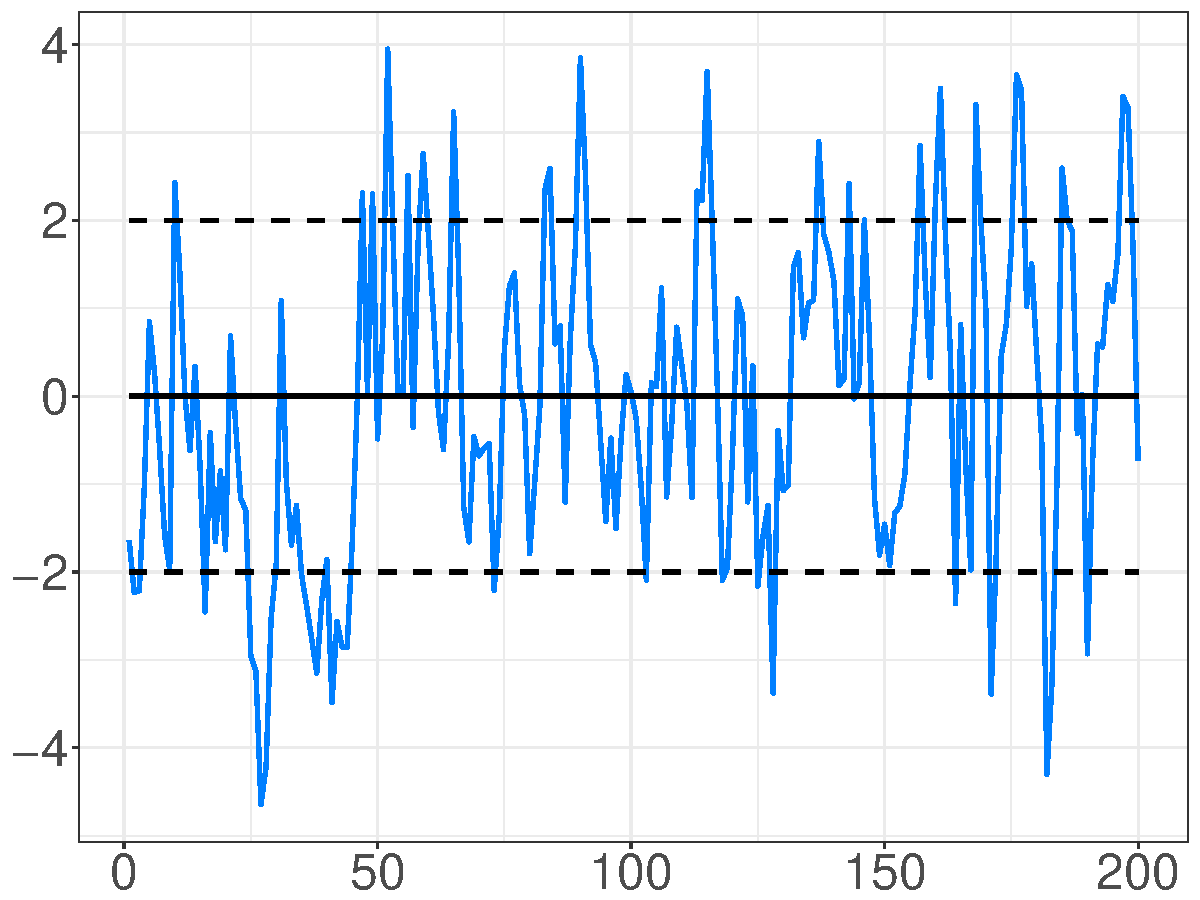
\includegraphics[width=1\linewidth]{images/stationary_ts.pdf}
 \caption{}
 \label{fig:stationary}
\end{subfigure}
\begin{subfigure}{.45\textwidth}
 \centering
 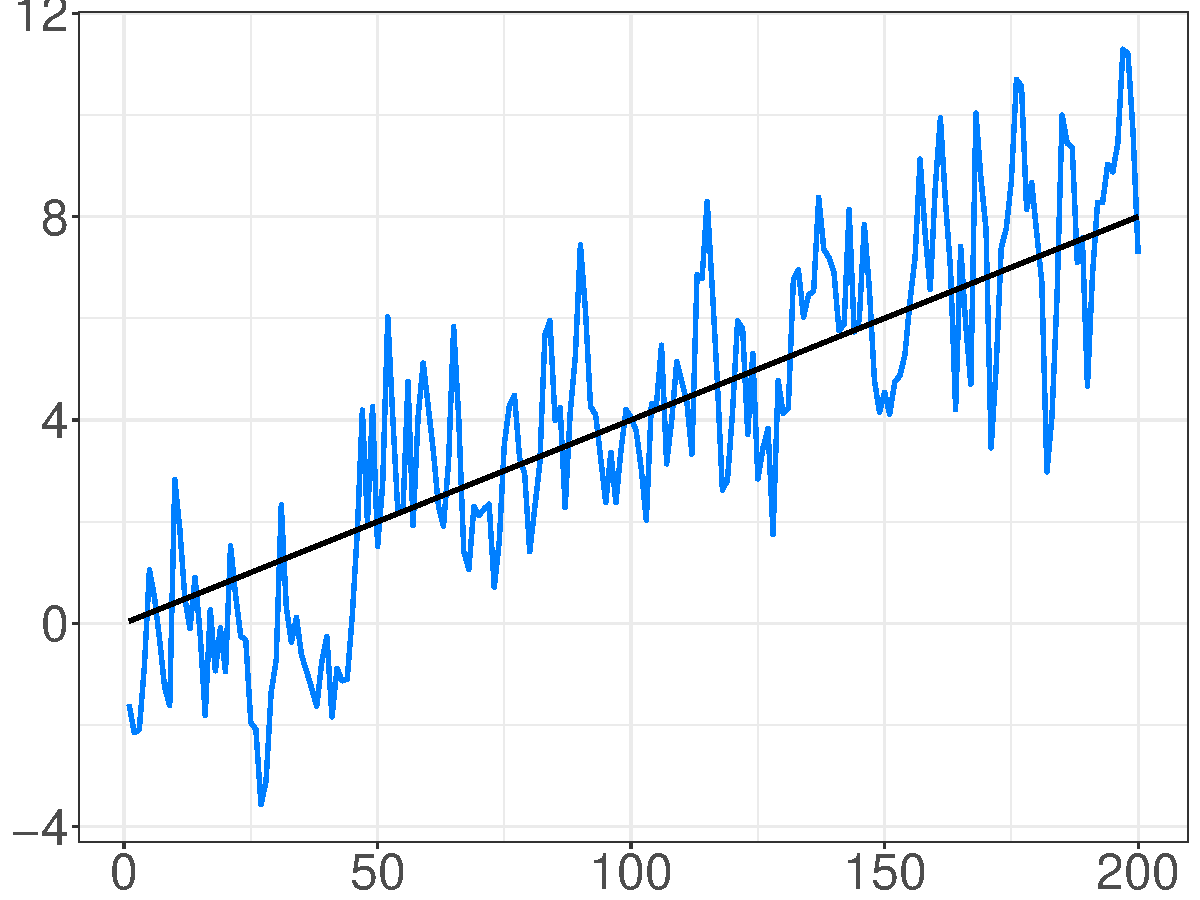
\includegraphics[width=1\linewidth]{images/trend-stationary_ts.pdf}
 \caption{}
 \label{fig:trend-stationary}
\end{subfigure}
\begin{subfigure}{.45\textwidth}
 \centering
 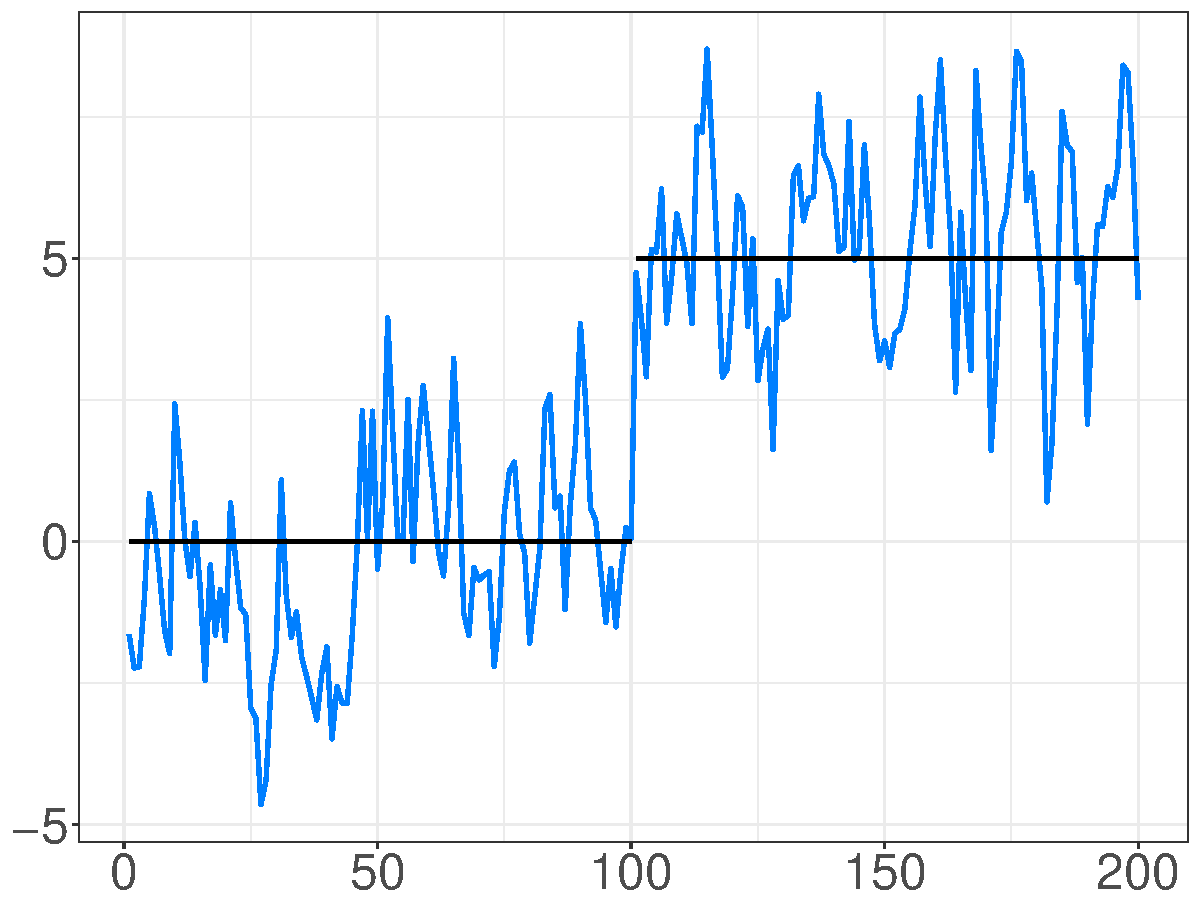
\includegraphics[width=1\linewidth]{images/level-stationary_ts.pdf}
 \caption{}
 \label{fig:level-stationary}
\end{subfigure}
\begin{subfigure}{.45\textwidth}
 \centering
 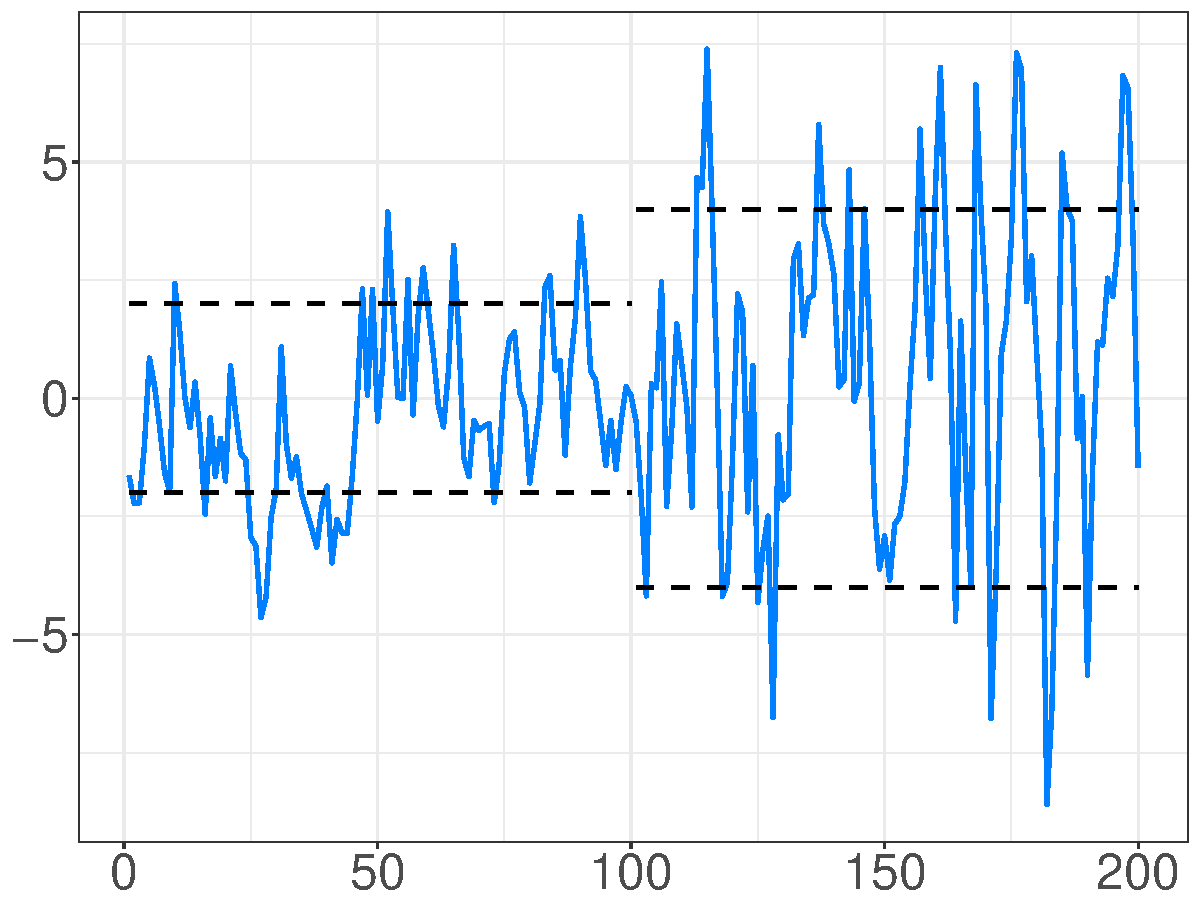
\includegraphics[width=1\linewidth]{images/heteroscedastic_ts.pdf}
 \caption{}
 \label{fig:heteroscedastic}
\end{subfigure}
\begin{subfigure}{.45\textwidth}
 \centering
 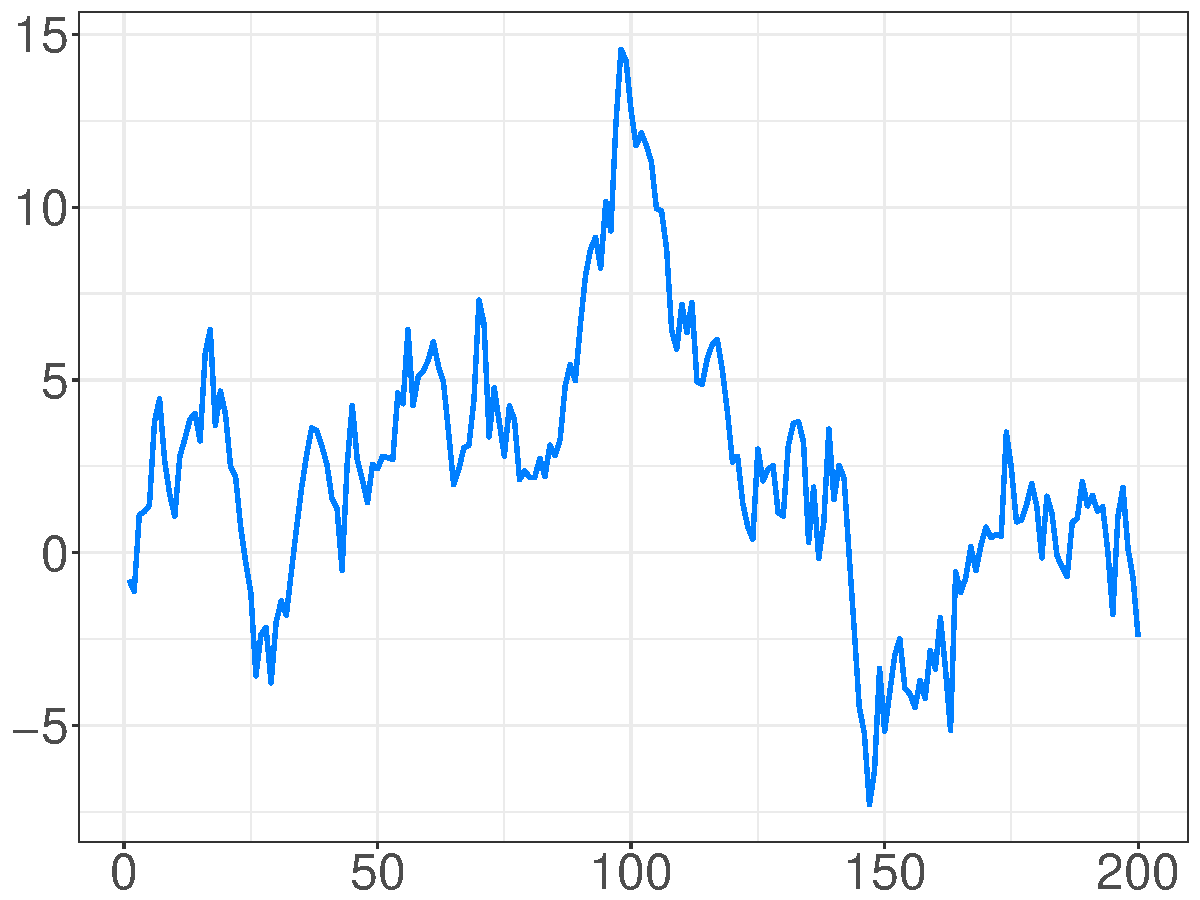
\includegraphics[width=1\linewidth]{images/difference-stationary_ts.pdf}
 \caption{}
 \label{fig:difference-stationary}
\end{subfigure}
\caption[Examples of nonstationary time series]{Examples of time series presenting the properties of (a) stationarity, and nonstationarity in the form of (b) trend stationarity, (c) level stationarity, (d) heteroscedasticity and (e) difference stationarity. The solid and dashed black lines represent the mean and the variance functions of the time series, respectively.}
\label{fig:nonstationarity}
\end{figure}

A trended model might be considered the simplest form of nonstationary time series. This model represents a process that has stationary behavior around a deterministic trend. This trend shifts the mean of a time series causing it to increase or decrease over time. Commonly, the deviations of a systematic trend may be a stationary variable, known as a detrended variable, which may be analyzed instead of the original time series. In that case, usual stationary models are applicable \cite{hanssens_market_2003,yang_nonstationarity_2010}. A time series that presents this behavior is called trend stationary. One may write an example model of such time series by adding a deterministic linear trend to the \acr{AR(1)} model presented in Equation~\ref{AR1}. This model is defined as in Equation~\ref{trendModel}, where ${\beta}t$ is the trend term and $\omega_t \sim N(0, \sigma^2_\omega)$ represents white noise.
The mean function of the process $E(x_t) = \mu_t = {\beta}t$ varies over time, violating the stationarity constraints. The time series represented in Equation~\ref{trendModel} may be observed in Figure~\ref{fig:trend-stationary} where one can see the linear increasing mean function. This model gives an example of a process which is nonstationary in mean.
\begin{equation}\label{trendModel}
x_t = \alpha + {\theta}x_{t-1} + {\beta}t + \omega_t, \ \ 0 < \theta < 1
\end{equation}

Nonstationarity in a time series may also be caused by structural breaks, that happen at specific points in time, usually due to environment changes. These structural breaks may eventually result in level shifts in a time series, which cause the mean function to be different for different portions of the series. In that case, a time series can be partitioned, and one can separately analyze each data portion with different statistical properties, provided that the timing of a structural break is known \cite{hanssens_market_2003}. Another way to handle structural breaks and level shifts in the mean function while modeling a time series is to make use of a dummy variable defined as zero before the point of a structural break and one after it. In case a time series presents local stationary properties on each different portion divided by a level shift it is known as being level stationary. An example of a level stationary time series is observed in Figure~\ref{fig:level-stationary} where one can see the level shifts of the mean function. The plot in Figure~\ref{fig:level-stationary} represents the model in Equation~\ref{levelModel} which is derived from Equation~\ref{AR1} by the addition of a dummy variable $d_t$, with the level shift $\delta = 5$ and the time of the structural break $t_b = 100$. This model gives another example of nonstationarity in the mean.
\begin{equation}\label{levelModel}
x_t = \alpha + {\theta}x_{t-1} + {\delta}d_t + \omega_t, \ \ 0 < \theta < 1, \ \ d_t = 
 \begin{cases}
 0, & \text{$t \le t_b$},\\
 1, & \text{$t > t_b$}.
 \end{cases}
\end{equation}

Another cause of nonstationarity which results from structural breaks is the change in variance over time, a condition which is commonly known as heteroscedasticity \cite{hanssens_market_2003,shumway_time_2017}. Heteroscedasticity arises from environment changes that make the volatility of time series observations increase/decrease over time. Time series which present this condition are called heteroscedastic. Analogous to level shifts, the different variance properties in different portions of a time series can be addressed by partitioning the series or by modeling the changes in variance with a dependency on the structural breakpoints. An example of heteroscedastic time series is depicted in Figure~\ref{fig:heteroscedastic} where different variance properties on the first and last portions of the series are easily observable. The series presented in Figure~\ref{fig:heteroscedastic} represent the same model defined in Equation~\ref{AR1} and the same series of Figure~\ref{fig:stationary}, but in this case, $\omega_t$ is set as $\omega_t \sim N(0, \sigma^2_\omega = 2)$ for $t = 1,\dots,100$ and $\omega_t \sim N(0, \sigma^2_\omega = 4)$ for $t = 101,\dots,200$. This model gives an example of a time series which presents nonstationarity in the variance.

An important type of nonstationarity, which in many cases is observed in real-world series, is caused by the presence of a unit root in the characteristic polynomial of a time series model. Without a unit root, time series observations tend to fluctuate around deterministic components such as a mean or a trend. Conversely, when a unit root is present, observations do not revert to a historical level and may wander in any direction. The presence of a unit root implies that the time series suffer from the influence of long-run components or stochastic trends \cite{hanssens_market_2003}. In that case, the removal of a stochastic trend, usually done by the application of a process called differencing, is often helpful to coerce such time series to stationarity. For that reason nonstationary time series that present unit roots are also known as difference stationary \cite{box_time_2008}. A difference stationary time series is presented in Figure~\ref{fig:difference-stationary} that represents the so-called random walk model, which can be formulated as in Equation~\ref{randomWalk}. This model assumes that the value of a time series $x_t$ at a time $t$ can be explained by the value of the series at the time $t - 1$ plus a random movement represented by $\omega_t$ \cite{shumway_time_2017}.
\begin{equation}\label{randomWalk}
x_t = \alpha + x_{t-1} + \omega_t = \alpha + \sum^{t}_{i=1}{\omega_i}
\end{equation}

The random walk model in Equation~\ref{randomWalk} is also derived from the \acr{AR(1)} model in Equation~\ref{AR1} by defining $\theta = 1$. The definition of $\theta = 1$ implies that any impacts caused by past observations result in a permanent effect on the global behavior of a time series. In this case, the mean function of the process is not fixed, and the variance function tends to increase over time \cite{hanssens_market_2003} as can be observed by Equation~\ref{randomWalkVAR}. This model gives an example of a process which presents a unit root and is nonstationary both in mean and in variance \cite{yang_nonstationarity_2010}.
\begin{equation}\label{randomWalkVAR}
VAR(x_t) = VAR(\alpha) + \sum^{t}_{i=1}{VAR(\omega_i)} = t\sigma^2_\omega \rightarrow \infty \ as \ t \rightarrow \infty
\end{equation}

It is also important to remark that frequently the dependence of a time series on past data may occur by multiples of some underlying seasonal lag $S$. In that case, a time series presents periodic components, and therefore, its statistical properties such as mean and variance may periodically change, creating a dependence on time $t$. This makes seasonality another particular form of nonstationarity, which is often found in time series \cite{yang_nonstationarity_2010}.

Generally, any form of nonstationarity, if not adequately addressed, can have a relevant impact on time series prediction applications. Overlooking nonstationarity properties in a time series may lead to misleading statistical inferences and bad or unexpected prediction results.

\chapter{Benchmarking framework}\label{framework}
\section{Usage examples} \label{usage}
This section gives examples for demonstrating the usage of the implemented framework for describing and performing a particular time series prediction application. The first example (Listing \ref{lst:ARIMA}) corresponds to a time series prediction using the \acr{ARIMA} model, which can be considered a benchmark linear model for such applications \cite{salles_framework_2017}.

\begin{lstlisting}[language=R, caption={[ARIMA model prediction application]R example for an ARIMA model prediction application using \textit{TSPred}}, label={lst:ARIMA}]

#loading TSPred package
 > loadlibrary("TSPred")

#loading CATS dataset
 > data("CATS")

#defining the time series application
 > tspred_arima <- tspred(
     subsetting = subsetting(test_len = 20),
     modeling = ARIMA(),
     evaluating = list(MSE = MSE(),AIC = AIC())
   )

#performing the prediction application and obtaining results
 > tspred_arima_res <- workflow(tspred_arima, data = CATS[3])
\end{lstlisting}

\chapter{Benchmarking of transformation methods}\label{experiment}

The research on the various nonstationary time series transformation methods reviewed in this work pointed to the relevancy of an experimental comparison of their practical effects in the time series prediction problem. Such comparison may shed light on the advantages and limitations of these methods in practical applications. It can help researchers analyze their best options for treating nonstationarity. This work fills this demand by devising and conducting a benchmarking process and comparative analysis of eleven of the reviewed transformation methods that are most commonly used in practical applications. The developed framework allowed the application of these methods in the prediction of time series of five different datasets originated from time series prediction competitions and real macroeconomic observations collected by a government institution. The datasets used in this experimental evaluation were made available. The next sections describe the performed experiment in detail and discuss its results.

\section{Datasets} \label{datasets}

Among the five time series datasets used in this experiment, three are benchmarks from time series prediction competitions (CATS \cite{lendasse_time_2007}, NN3 \cite{nn3_nn3_2007}, and NN5 \cite{nn5_nn5_2008}). The other two datasets are provided by the \acr{Ipea} \cite{ipea_ipeadata._2017} and are derived from real economic and financial data of the world. When selecting these datasets, the aim was to obtain a reasonable number of representative time series presenting different types of nonstationarity and statistical properties to provide a discussion on the effects of the evaluated transformation methods applied to the prediction of a diverse range of time series.

Moreover, this choice of datasets was made so as to encompass all domains of application of the publications reviewed. Particularly, the CATS dataset represents the statistical/natural sciences domain, the NN3 and NN5 datasets represent the industrial/business domain, and the datasets provided by \acr{Ipea} represent the socioeconomic/financial domain. 

The CATS Competition dataset presents an artificial time series with 5,000 observations, among which 100 are unknown. The unknown observations are grouped into five non-consecutive gaps of 20 successive values. The prediction of each gap may be considered a different problem, and each subset of the series followed by a gap may be considered a different time series to be modeled. In this context, the CATS dataset was considered as being composed of five time series of 980 observations. Both the NN3 and the NN5 Competition datasets present 111 time series. The series from the NN3 dataset have from 50 to 126 monthly observations drawn from a homogeneous population of real empirical business time series. All series from the NN5 dataset have 735 observations originated from daily withdrawals at 111 different cash machines within England, and may present missing data.

The two time series datasets provided by \acr{Ipea} were selected as the most requested series collected in monthly and daily rates, and are henceforth referenced as Ipea\_M and Ipea\_D datasets, respectively. The \acr{Ipea} is a public institution of Brazil that provides support to the federal government concerning public policies: fiscal, social, and economic. The data collected by \acr{Ipea} and used in this experiment comprehend information on exchange rates (R\$/US\$), exports/imports prices, interest rates, minimum wage, unemployment rate, and more, measured from 1930 to September of 2017. Ipea\_M contains 23 time series of 156 to 1019 observations. Ipea\_D contains 12 time series of 901 to 8154 observations.

In order to obtain a better understanding of the statistical properties of the selected time series datasets, 7 of the most common statistical tests have been performed for autocorrelation, randomness and independence, heteroscedasticity, linearity, and stationarity. Table \ref{tb:statsprop} contains a summary of the results of the statistical tests. For each dataset, it is presented the percentage of time series that had the null hypothesis test ($H_0$) confirmed.

\begin{table}[!ht]
    \centering
    \caption{Statistical tests results and analysis}
    \label{tb:statsprop}
        \begin{center}
\setlength{\tabcolsep}{4pt}
            \begin{tabular}{@{}llccccc@{}}
                \toprule
                \multicolumn{1}{c}{Statistical Tests} & \multicolumn{1}{c}{H0} & \multicolumn{1}{c}{CATS} & \multicolumn{1}{c}{NN3} & \multicolumn{1}{c}{NN5} & \multicolumn{1}{c}{Ipea\_M} & \multicolumn{1}{c}{Ipea\_D} \\ \midrule
                Breusch-Godfrey & Uncorrelated residuals & 0\% & 37\% & 0\% & 0\% & 0\% \\
                Box-Pierce & Randomness & 0\% & 30\% & 0\% & 0\% & 0\% \\
                Goldfeld-Quandt & Homoscedasticity & 40\% & 91\% & 48\% & 70\% & 50\% \\
                White Neural Network & Linearity in mean & 100\% & 81\% & 59\% & 83\% & 75\% \\
                ADF$^1$ & Nonstationarity & 100\% & 62\% & 5\% & 100\% & 58\% \\
                KPSS$^2$ & Trend Stationarity & 0\% & 70\% & 71\% & 4\% & 8\% \\
                KPSS$^2$ & Level Stationarity & 0\% & 57\% & 50\% & 4\% & 0\% \\ \bottomrule
            \end{tabular}
        \end{center}
        \footnotesize\emph{$^1$}Augmented Dickey-Fuller\\
        \emph{$^2$}Kwiatkowski-Phillips-Schmidt-Shin
\end{table}

The results in Table \ref{tb:statsprop} show the considerable disparity in the statistical properties of the time series in the selected datasets. It is possible to observe that most time series did not confirm the null hypothesis of uncorrelated residuals and randomness. The heteroscedastic and linearity tests indicate that a substantial number of the time series present the properties of homoscedasticity and linear behavior around the mean. This result means that one can expect relative stability in the variance of the time series. Finally, the stationarity tests results show that a considerable amount of the time series over all datasets is nonstationary presenting unit root (also known as difference stationary), trend stationary (stationary around a deterministic trend) or level stationary (stationary around a level that changes over time). These latter results are particularly favorable for motivating the application of transformation methods such as the previously described in this work.

\chapter{Enabling the benchmarking of transformation methods and models}\label{experiment2}
\section{Use case 1: choice of hyperparameters} \label{uc1}
\begin{Ualgorithm}[ht!]
	\KwIn{
		$X=$ experimental time series data\;
		$m=$ number of observations to be predicted\;
		$A=$ set of parameter combinations\
	}
	\KwOut{\
		$\hat{\alpha}=$ selected hyperparameter candidate\
	}
	\SetNlSkip{1em}
	\SetAlgoVlined\SetArgSty{}
	\Begin{$X_{eval} \gets \text{DataSampling}(X, m)$\;
		$X_{train} \gets X - X_{eval}$\;
		\
		\ForEach{parameter combination $\alpha$ in $A$}{
			$\mu_\alpha \gets \text{TrainMLP}(X_{train},\alpha)$\;
			$\rho_\alpha \gets \text{Predict}(\mu_\alpha,X_{train},m)$\;
			$\epsilon_\alpha \gets \text{Evaluate}(\rho_\alpha,X_{eval})$\;
			$\epsilon_A \gets \text{Append}(\epsilon_A,\epsilon_\alpha)$\;
		}
		$R \gets \text{Benchmark}(\epsilon_A,A)$\;
		$\hat{\alpha} \gets \text{Top1}(R)$\
	}
	\caption{Experimental methodology of use case 1}\label{alg_uc1}
\end{Ualgorithm}

\addcontentsline{toc}{chapter}{Final considerations}
\chapter*{Final considerations}\label{conclusion}

This work focus on the study of univariate nonstationary time series prediction and the benchmarking of preprocessing and modeling options for time series applications that have nonstationarity as an inherent property.
It is presented a review of nonstationary time series transformation methods for time series prediction. A categorization of such transformation methods was described together with a timeline obtained through a systematic mapping study. Moreover, it was developed a systematic framework for benchmarking transformation methods and models for nonstationary time series prediction. This framework was implemented and encapsulated within the \emph{TSPred} R-package \cite{salles_tspred:_2018}, which is publicly available.

The developed benchmarking framework was adopted for devising a comparative experimental analysis and discussion of the effects of some of the reviewed transformation methods on the problem of time series prediction. With this intent, eleven methods of the most commonly used in practical applications were selected and benchmarked. The aim of this experimental analysis is contributing to the process of evaluation, selection, and application of nonstationary time series transformation methods.

An overview of the effects of the evaluated methods regarding predictions and stationarity was produced based on our experimental results. Although it was possible to note a somewhat consistency in the results of the evaluated transformation methods, there was no uniquely best method across all datasets, and the nature and statistical properties of the time series were especially relevant to the results.

Nonetheless, it was possible to observe better predictions when transformation methods based on differencing and moving average smoothing were applied before the prediction of the time series of the selected datasets. Transformation methods that perform time series decomposition, which have been an object of increasing attention, were also among the best methods. Among the worst methods was, as expected, the naive one, where no data transformation is performed before prediction. Particularly, this approach provided predictions with significantly lower accuracy when compared to the case in which nonstationarity was treated.

Additionally, results indicate that the use of a validation phase for exploring different transformation methods generally leads to the selection of one of the most appropriate for obtaining accurate time series predictions. Our experimental results suggest as future trends (i) the increase in the importance of the process of data transformation for the problem of accurate prediction of nonstationary time series and (ii) the need for studying and evaluating suitable methods to perform this activity according to the dataset at hand.

In this context, the potential of the developed framework for enabling the benchmarking of data transformation methods and prediction models for a particular nonstationary time series application was indicated. With this goal, this work presents use case examples of the framework usability encompassing the selection of hyperparameters, and the choice of adequate transformation methods and machine learning prediction models. For example purposes, the use cases benchmark the top 5 evaluated transformation methods and six different \acr{MLM} for prediction of 5 selected nonstationary time series. The benchmark linear \acr{ARIMA} model is also adopted to indicate demands for the refining of preprocessing methods and model parameters. Results are analyzed and the general methodologies for benchmarking and selecting adequate prediction setups for a particular nonstationary time series are described.

\addcontentsline{toc}{section}{Scientific production}
\section*{Scientific production}

The study conducted around the topic of nonstationary time series prediction resulted in the publication of four main scientific research products \cite{salles_evaluating_2016,salles_framework_2017,salles_tspred:_2018,salles_nonstationary_2019}. The paper of \textcite{salles_evaluating_2016} was published in the Ecological Informatics journal. It performs an experimental analysis of time series predictions based on nonstationary sensor data of the sea surface temperature (SST) of the tropical Atlantic ocean. The data is collected by the Prediction and Research Moored Array in the Tropical Atlantic (PIRATA) project \cite{goos-brasil_pirata_2015}. The paper focused on evaluating the influence of temporal aggregation in predicting step-ahead SST considering different prediction horizons and different sizes for training datasets. Results point out scenarios indicating whether or not temporal aggregated SST time series may be beneficial for prediction. The improvement of SST prediction is important for aiding the identification of extreme environmental events such as droughts.

The paper of \textcite{salles_framework_2017} was published in the proceedings of the International Joint Conference on Neural Networks (IJCNN) held at Anchorage, Alaska, USA. It presents a framework for systematic benchmarking \acr{MLM} against well-known \acr{LM}, namely Polynomial Regression and models in the \acr{ARIMA} family, used as benchmark models for univariate time series prediction. This implementation was evaluated using a wide number of datasets from past prediction competitions. The results showed that fittest \acr{LM} provided by the framework are adequate benchmark models for performance assessment of univariate time series predictions.

The scientific research content presented in this text was also published and is currently available. The framework described in Chapter \ref{framework} automatizes the time series prediction process including the tasks of data preprocessing, modeling, prediction, data postprocessing and the evaluation of prediction quality. Several methods related to each of these tasks are implemented with the incorporation of automatic choice of parameters. Moreover, the structure of the framework was designed for supporting the custom user implementation of methods in a straightforward manner.

The framework offers tools for benchmarking different preprocessing methods and models for the prediction of nonstationary time series of a particular application. Being widely available within the \emph{TSPred} R-package \cite{salles_tspred:_2018} in \acr{CRAN}, the potential for application of this framework encompasses the areas of statistical sciences, natural sciences, socioeconomics, finance, industry and business. By the end of 2018, the previous version 4.0 of \emph{TSPred} had an average of $680$ downloads per month worldwide. Given its comprehensiveness and practical use, it is expected that the advent of its new version 5.0, incorporating the described framework, brings a significantly higher utilization rate.

Finally, the review and experimental analysis of nonstationary time series transformation methods presented in this text (Chapters \ref{TSandNonstat} and \ref{experiment}) were published in the journal Knowledge-Based Systems \cite{salles_nonstationary_2019}. The paper focused on contributing to the choice of a transformation that is appropriate to the adopted data model and to the problem at hand. It provides a background on the subject of nonstationary time series transformation methods and a discussion on the scenarios they could be most beneficial to the problem of time series prediction.

%-----------------------------------------------
% References
%-----------------------------------------------

\addcontentsline{toc}{chapter}{References}
\printbibliography
\end{document}
